
\section{Heavy flavour process in \texorpdfstring{\znunu}{Zinv}+jets}
\label{sec:zplusbb_app}

To investigate the effect of potential simulation mismodelling on
processes involving the production Z bosons and b-quarks (\ie
associated b-quark production or gluon splitting), the background
expectations in all bins of the \mmj control region, as determined
from simulation, are divided into two ``templates'' based on
generator-level information: the first contains the ``heavy flavour''
Z + b and Z + gluon($\ra$bb) processes, the second contains
all other ``light flavour'' processes involving Z production. The
partial cross sections for the two sets of processes (templates) are
floated in a fit to extract the ``signal strength'' correction
$\mu_\mathrm{HF}$. The fit is performed in the \mmj control region,
assumed to be a valid proxy for the \znunu + (b)jets background in the
signal region. A likelihood is constructed with all experimental and 
theoretical uncertainties relevant to the \mmj control region. The fit
is performed for the run eras G-H dataset. The maximum-likelihood
value for $\mu_\mathrm{HF}$ is $1.10 \pm 0.46$.

A further two fits are performed, for which the partial cross section
for the heavy flavour processes is varied first by a factor of 0.5,
and then by a factor 2. The effect on the b-tag-related nuisances can
be seen in Figure~\ref{fig:zplusbb}, which demonstrates pulls of
$<1\sigma$

\begin{figure}[h!]
  \centering
  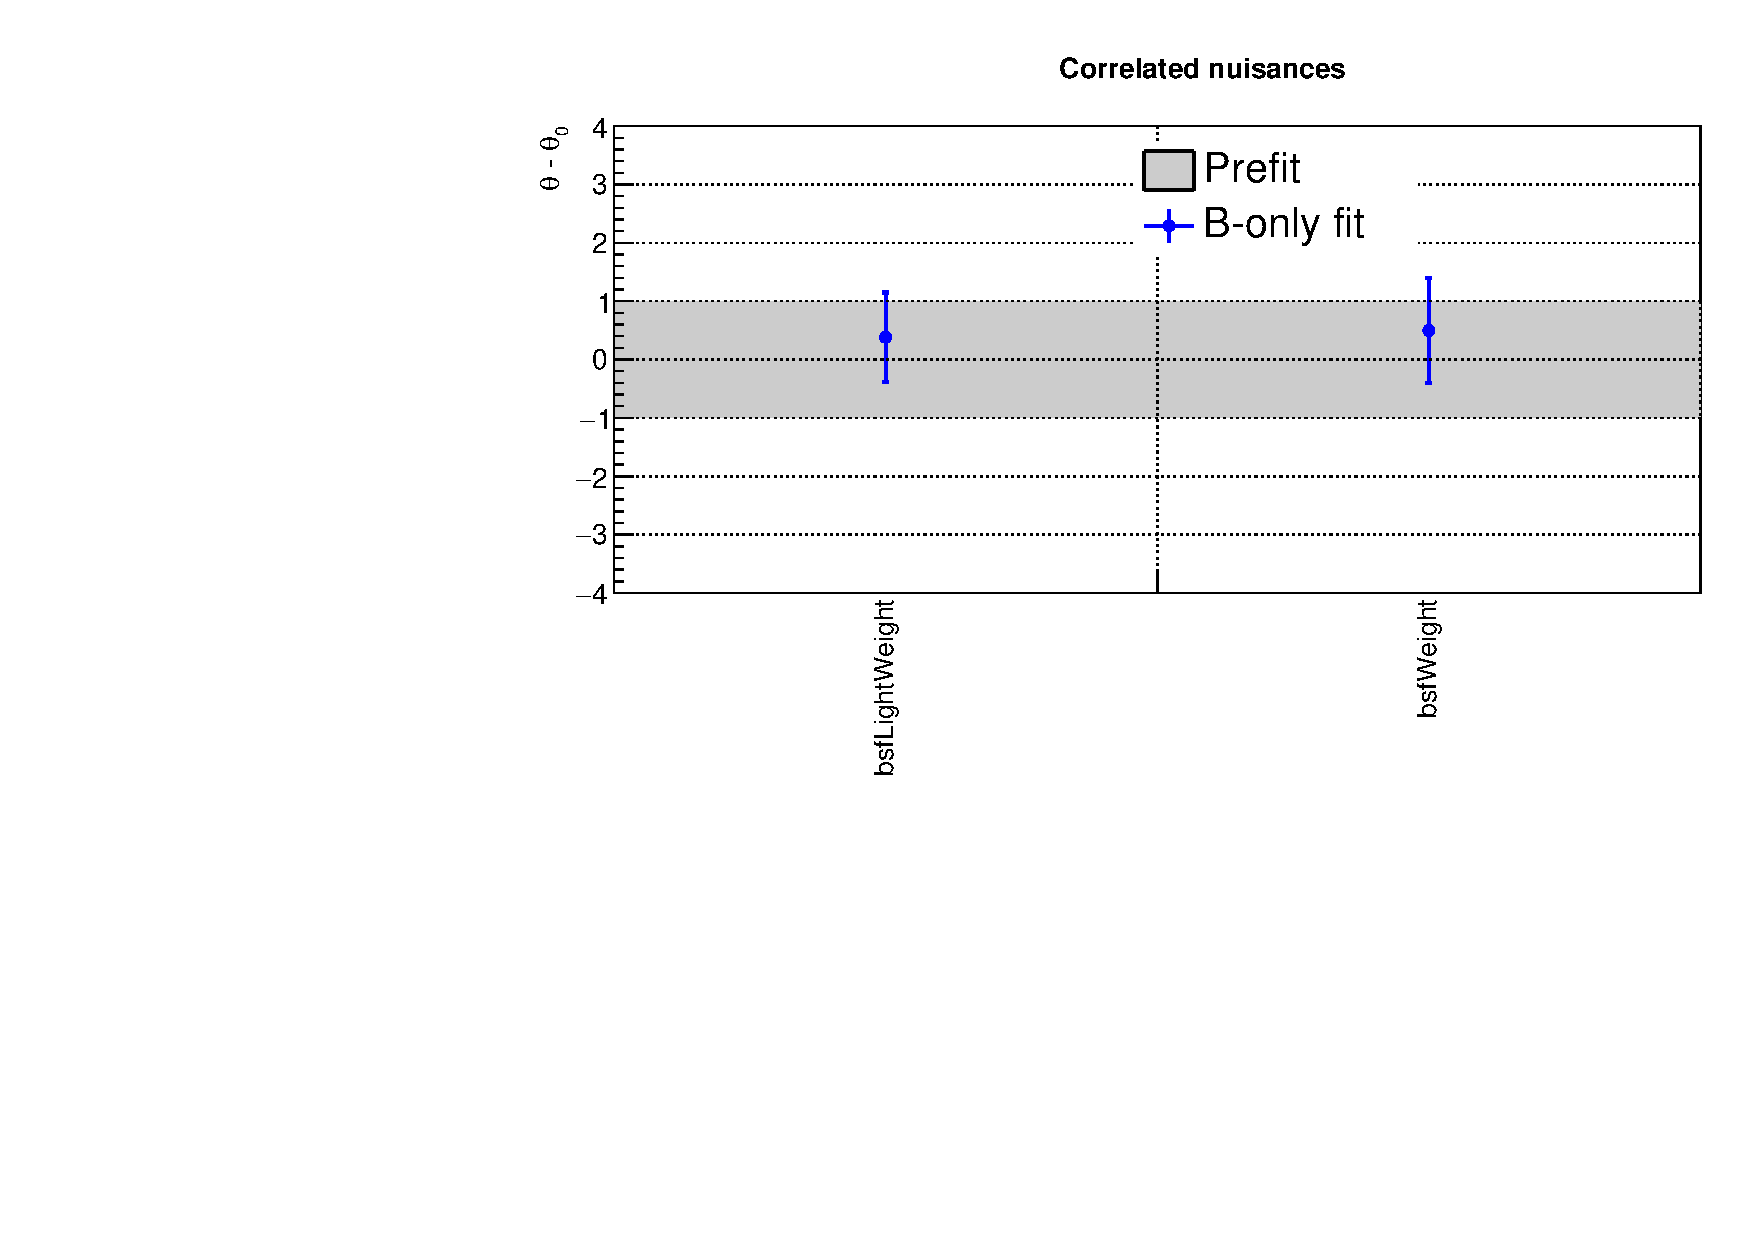
\includegraphics[width=0.6\textwidth]{figures/ZPlusbb/TemplateFitv1_HFXs0p5}
  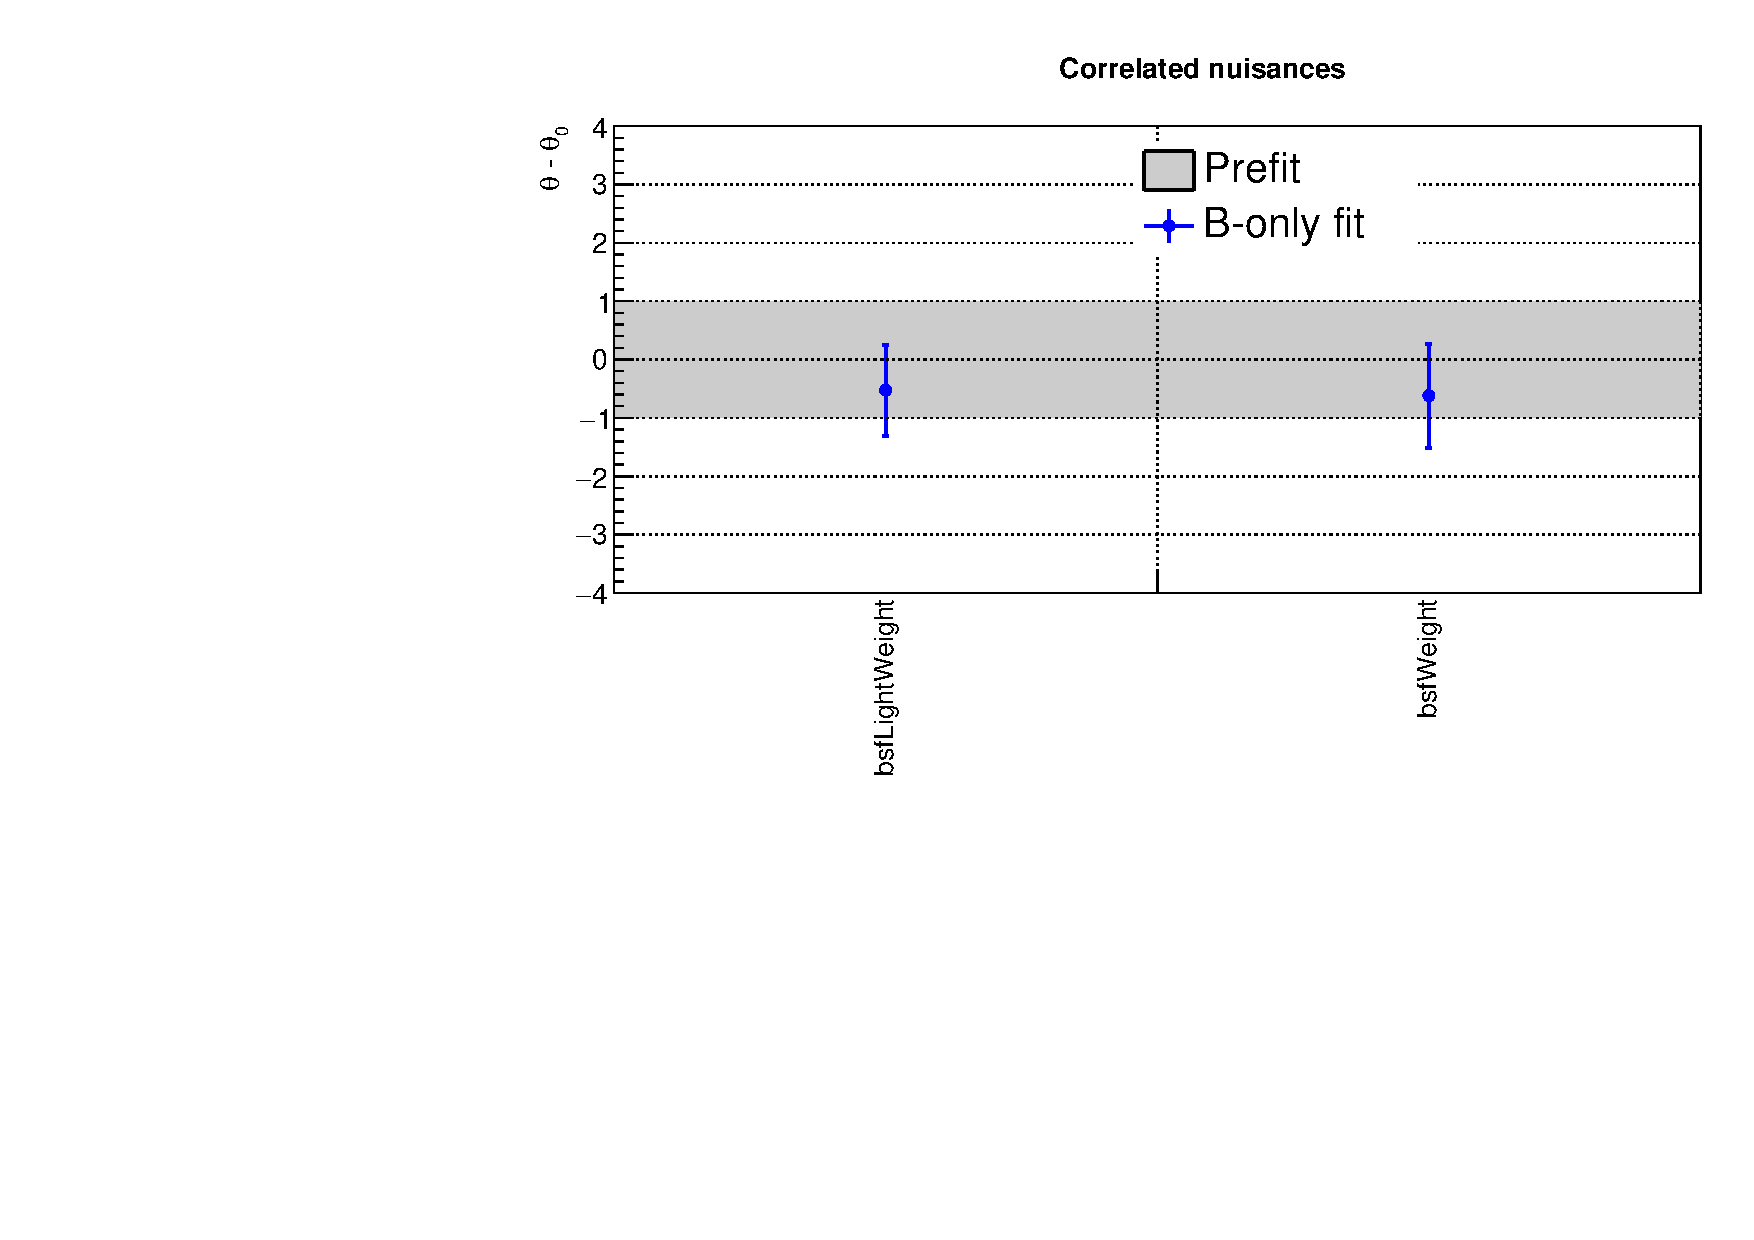
\includegraphics[width=0.6\textwidth]{figures/ZPlusbb/TemplateFitv1_HFXs2p0}
  \caption{\label{fig:btagsfge1b} Post-fit nuisances of a likelihood
    fit to data in the \mmj control region with scaling the cross section of heavy 
    flavour process by a factor of 0.5 (top) and 2.0 (bottom). }
  \label{fig:zplusbb}
\end{figure}

\begin{figure}[h!]
  \centering
  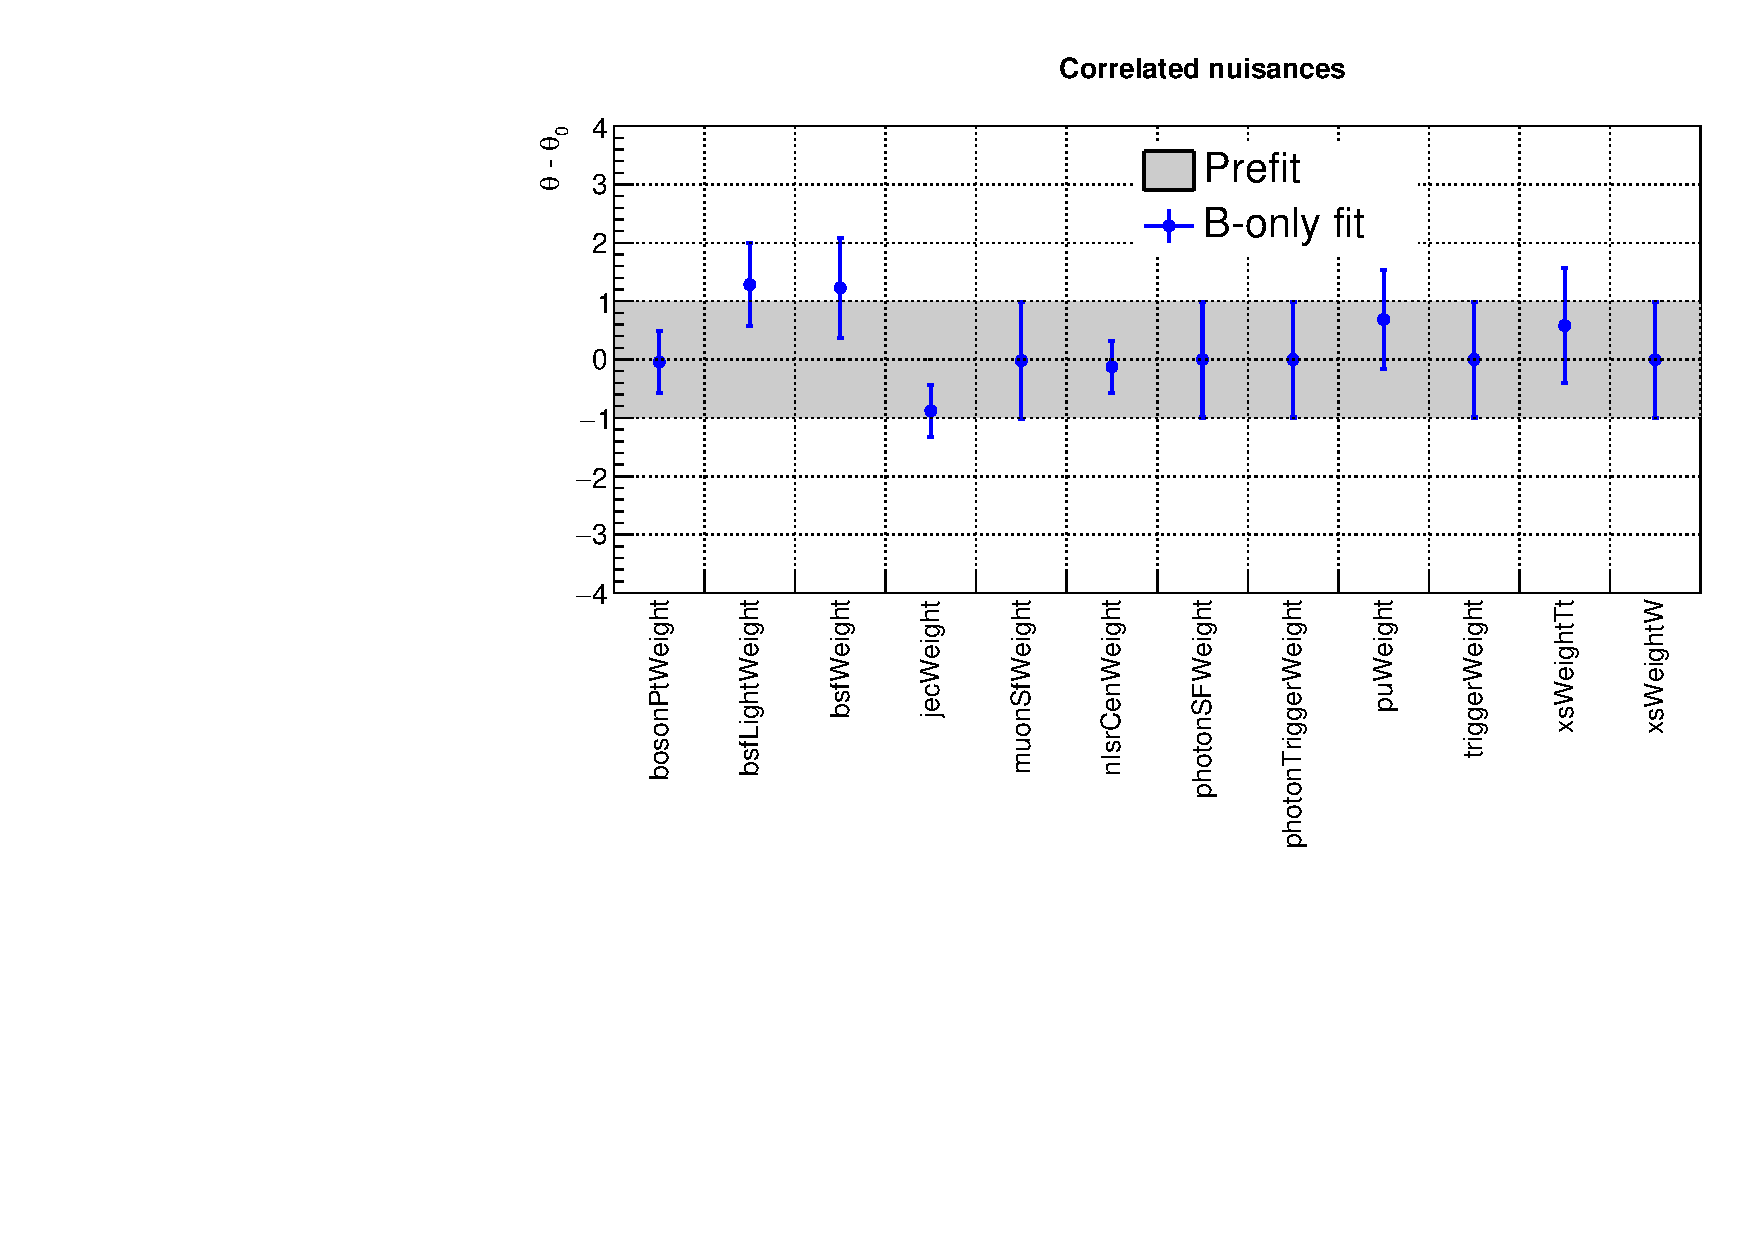
\includegraphics[width=0.6\textwidth]{figures/ZPlusbb/TemplateFitv2_36invfb}
  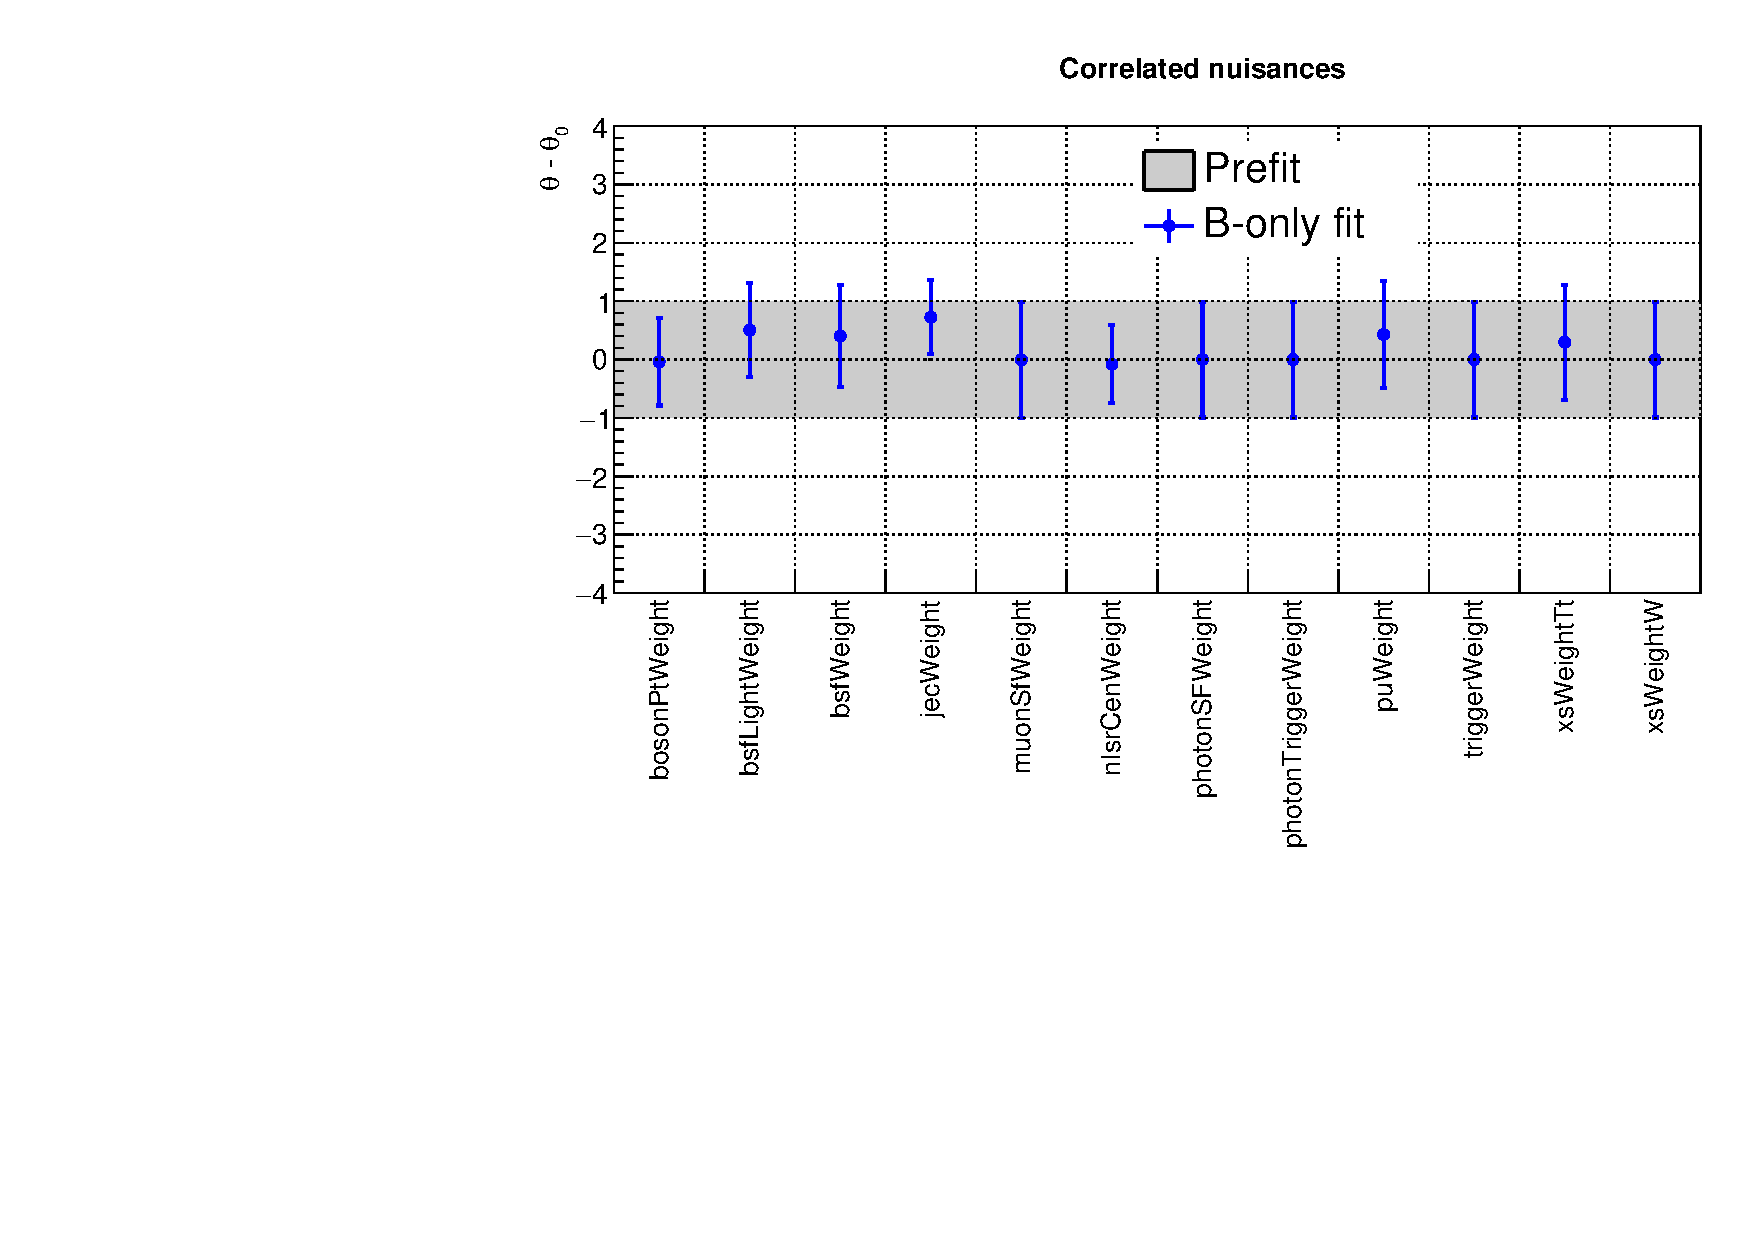
\includegraphics[width=0.6\textwidth]{figures/ZPlusbb/TemplateFitv2_16invfb}
  \caption{\label{fig:btagsfge1b} Post-fit nuisances of likelihood
    fits to data in the \mmj control region to extract heavy flavour 
    cross section, with full dataset with 35.9 \ifb (top) and partial dataset 
    G-H with 16.6 \ifb (bottom).}
  \label{fig:zplusbb2}
\end{figure}

